\chapter{Computational Details}
This chapter provides the details of the computational methods used in this work. The first section describes the generation of the training dataset, including the preparation of the system, initial equilibration using the molecular mechanics, exploration of the configuration space at the xTB level, further data labeling, and iterative training of the neural network potential. The second section discusses the production runs at different temperatures using the fitted neural network potential. The third section describes the workflow of validating the transition states obtained from the simulations following the partial Hessian formalism. Finally, the fourth section presents the data analysis and visualisation techniques employed to interpret the results.

%%%%%%%%%%%%%%%%%%%%%%%%%%%%%%%%%%%%%%%%%%%%%%%%%%%%%%%%%%%%%%%%%%%%%%%%%%%%%%%%

\section{Training dataset generation}

\subsection{System preparation}
The systems were prepared using the CHARMM-GUI webserver's functionality \citep{joCHARMMGUIWebbasedGraphical2008}. In particular, the Multicomponent Assembler interface \citep{kernCHARMMGUIMulticomponentAssembler2024} was utilised. 

As a first step, the singly protonated and deprotonated forms of the methyl diphosphate were parametrised in CGenFF \citep{kimCHARMMGUILigandReader2017}, i.e. CHARMM General Forcefield. These states of the methyl diphosphate were chosen based on the fact that pyrophosphoric (diphosphoric) acid has the following dissociation constants \citep{haynesCRCHandbookChemistry2016}:
\begin{align*}
    \mathrm{H_4P_2O_7} \rightleftharpoons \mathrm{[H_3P_2O_7]^-} + \mathrm{H^+},\quad \mathrm{p}K_\mathrm{a} = 0.91 \\
    \mathrm{[H_3P_2O_7]^-} \rightleftharpoons \mathrm{[H_2P_2O_7]^{2-}} + \mathrm{H^+},\quad \mathrm{p}K_\mathrm{a} = 2.10 \\
    \mathrm{[H_2P_2O_7]^{2-}} \rightleftharpoons \mathrm{[HP_2O_7]^{3-}} + \mathrm{H^+},\quad \mathrm{p}K_\mathrm{a} = 6.70 \\
    \mathrm{[HP_2O_7]^{3-}} \rightleftharpoons \mathrm{[P_2O_7]^{4-}} + \mathrm{H^+},\quad \mathrm{p}K_\mathrm{a} = 9.32
\end{align*}
Thus, at the physiological pH of 7.4 this acid exists as an equillibrium between the doubly and singly protonated forms. As an assumption, the methyl group can be considered as a proton, therefore we condsidered the methyl diphosphate molecule to exist as a mixture of the singly (MeHDP) and deprotonated (MeDP) forms at the physiological pH.

After succesfully parametrising the molecules, the system was solvated in a cubic box of TIP3 water molecules together with the sodium counterions Na\textsuperscript{+} to neutralise the charge. The final system composition can be seen in Table \ref{tab:system-before-equilibration}.

\subsection{Initial equilibration using the classical forcefields}
The equilibration of the system was performed following the standard protocol generated by the CHARMM-GUI webserver \citep{joCHARMMGUIWebbasedGraphical2008}. The system was first energy minimised using the steepest descent algorithm for 5000 steps. 

Subsequently the system was equillibrated in the NVT (constant number of particles, volume, and temperature) ensemble for 5 ns. During the minimisation and NVT equilibration, the heavy atoms of the solute were restrained using a harmonic potential with a force constant of 400 kJ mol\textsuperscript{-1} nm\textsuperscript{-2}.

As a last step, the system was equilibrated in the NPT (constant number of particles, pressure, and temperature) ensemble for 45 ns. Throughout the whole protocol, the temperature was set to 300 K and the pressure was set to 1 bar. To ensure the constant temperature and pressure, the system was coupled to a $\nu$-rescale thermostat \citep{bussiCanonicalSamplingVelocity2007} with a coupling constant of 1 ps and an isotropic \textit{c}-rescale barostat \citep{bernettiPressureControlUsing2020} with a coupling constant of 5 ps. During the NPT run, the cut-off for the non-bonded interactions was set to 0.6 nm and the long-range electrostatics were treated using the Particle Mesh Ewald (PME) method.  In all steps, the periodic boundary conditions (PBC) were applied in all directions.
\begin{table}[b]
    \centering
    \caption{System composition and simulation box details.}
    \label{tab:system-before-equilibration}
    \begin{tabular}{lccc}
    \toprule
    \textbf{System} & \textbf{Equillibrated box dimensions (\AA\textsuperscript{3})} & \textbf{No. of H\textsubscript{2}O} & \textbf{No. of Na\textsuperscript{+}} \\
    \midrule
    MeDP  & $15.877 \times 15.877 \times 15.877$ & 119 & 3 \\
    MeHDP & $15.901 \times 15.901 \times 15.901$ & 124 & 2 \\
    \bottomrule
    \end{tabular}
\end{table}

All simulations were conducted in GROMACS 2021.4 \citep{abrahamGROMACSHighPerformance2015} using the CHARMM36m forcefield \citep{huangCHARMM36mImprovedForce2017} and the leap-frog integration method with a time step of 1 fs. All hydrogen involving bonds were constrained using the LINCS algorithm. The final dimensions of the box for all further calculations were obtained after the NPT run and are shown in Table \ref{tab:system-before-equilibration}. The last frame of the NPT runs was used as a starting point in all further calculations unless stated otherwise.



\subsection{Collective variables}
In order to properly sample the reaction space, we used two types of collective variables (CVs) to bias the system, e.g. distances and coordination numbers (CNs). The coordination number is defined as the smooth coordination number function:
\begin{equation}
    \sum_{i \in A} \sum_{j \in B} CN_{ij} = \frac{1 - \left( \frac{r_{ij} - d_0}{r_0} \right)^n}{1 - \left( \frac{r_{ij} - d_0}{r_0} \right)^m}
    \label{eq:coordination_number}
\end{equation}
where $r_{ij}$ is the distance between the atoms $i$ and $j$ from the groups $A$ and $B$, $d_0$ is a shift in the distance where CN starts to decay, $r_0$ is a scaling parameter or a characteristic decay length that defines how fast the CN drops off with distance, and $n$ and $m$ are the positive integers that control the steepness of the function. Normally, $m > n$ and the purpose of these parameters is to control how quickly the neighbours stop contributing as the distance increases. Therefore, the $CN_{ij}$ ranges from $\approx1$ when $r_{ij} \le r_0$ and $\approx0$ when $r_{ij} \ge r_0$. The CVs used to bias the systems in this work are shown in Figure \ref{fig:collective_variables}. The corresponding parameters to describe each collective variable are as follows:

\begin{itemize}
    \item The distance between the $\beta$-phosphorus and the oxygen atom connecting it to the rest of the molecule (CV\textsubscript{1}, d(O\textsubscript{remaining} - P\textsubscript{leaving}),
    \item The coordination number of all oxygens around the $\beta$-phosphorus atom (CV\textsubscript{2}, CN(P\textsubscript{leaving} - O\textsubscript{all})): $d_0 = 0$, $r_0 = 2.1$ \AA, $n = 8$, $m = 16$,
    \item The coordination number of all hydrogens excluding the methyl ones around the oxygen atoms bound to the $\beta$-phosphorus atom (CV\textsubscript{3}, CN(O\textsubscript{leaving} - H\textsubscript{all})): $d_0 = 0$, $r_0 = 1.4$ \AA, $n = 6$, $m = 12$.
\end{itemize}

Besides the above mentioned CVs that were biased during the simulations, we also used the following collective variables to track the number of H\textsubscript{3}O\textsuperscript{+} and OH\textsuperscript{-} in the solution:
\begin{itemize}
    \item The number of H\textsubscript{3}O\textsuperscript{+} (n\textsubscript{H\textsubscript{3}O\textsuperscript{+}}): TODO,
    \item The number of OH\textsuperscript{-} (n\textsubscript{OH\textsuperscript{-}}): TODO.
\end{itemize}

\begin{figure}[t!]
    \centering
    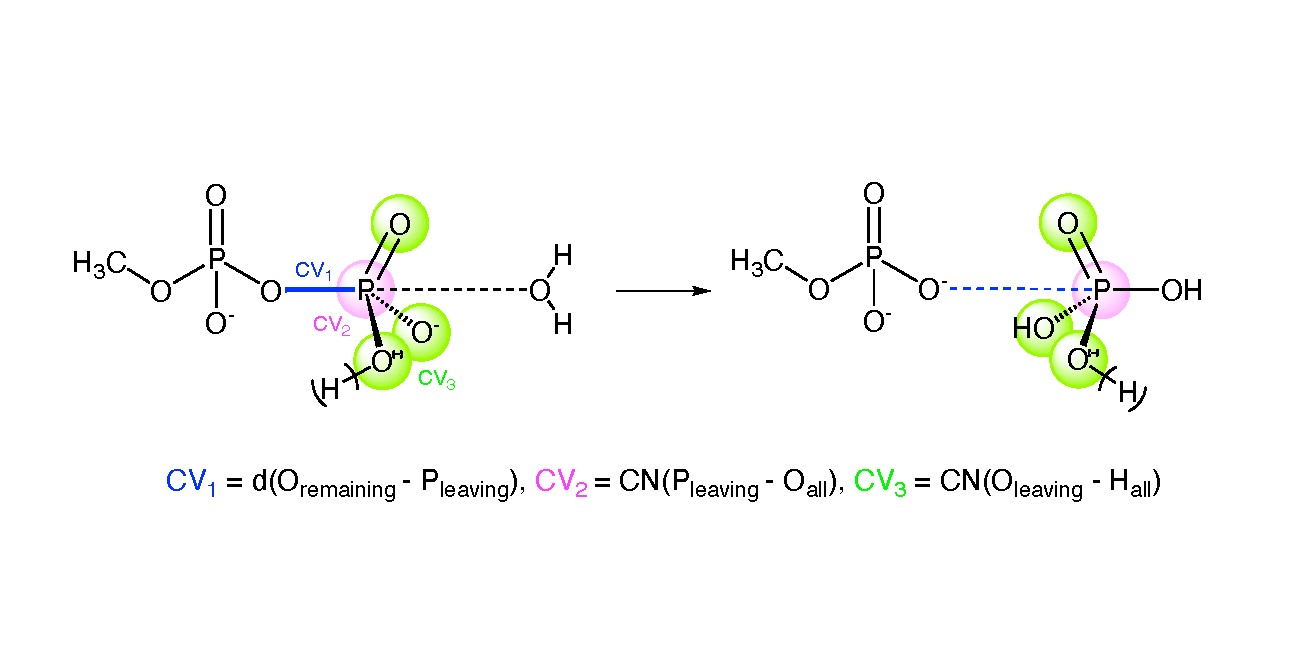
\includegraphics[width=0.95\textwidth]{Figures/3_Computational_details/collective_variables.pdf}
    \caption{The definition of the collective variables (CVs) used in this work. CN stands for the coordination number.}
    \label{fig:collective_variables}
\end{figure}

To prevent the system from exploring the unphysical regions of the potential energy surface, we additionally applied quadratic (harmonic-like) wall potentials to softly restrain the accessible regions of some of the degrees of freedom. 

The aforementioned wall potentials have the following form:
\begin{equation}
    \text{for upper walls:} \; \sum_i k_i \left( \frac{CV_i - a_i + o_i}{s_i} \right)^{e_i}
    \label{eq:upper_wall}
\end{equation}
\begin{equation}
    \text{for lower walls:} \; \sum_i k_i \left| \frac{CV_i - a_i - o_i}{s_i} \right|^{e_i}
    \label{eq:lower_wall}
\end{equation}
where $CV_i$ is the value of the collective variable, $k_i$ is the force constant (wall strength) that controls how strong the wall pushes back, $a_i$ is the position of the wall, $o_i$ is the offset to shift the wall slightly, $s_i$ is the rescaling factor, and $e_i$ is the exponent that determines the sharpness of the wall. When $e_i = 2$ the wall is harmonic-like. 

Thus this potential is equal to zero while the CV is within the boundaries but once the CV tries to go beyond the boundaries, the potential increases and penalises the system.

The wall potentials were applied to the following collective variables:
\begin{itemize}
    \item CV\textsubscript{1}, d(O\textsubscript{remaining} - P\textsubscript{leaving}): $k = 500$ kcal mol\textsuperscript{-1} \AA\textsuperscript{-2}, $a = 5.0$ \AA (upper wall), $o = 0$ \AA, $s = 1$ \AA, $e = 2$),
    \item TODO (CONSIDER TRANSFORMING INTO A TABLE)
\end{itemize}

All CV related computations were carried out using either the CP2K 2023.1 in-built tools \citep{kuhneCP2KElectronicStructure2020} or PLUMED 2.9.3 \citep{tribelloPLUMED2New2014}. It's important to note that the number of the CVs and the restraints used in the simulations varies depending on the part of the overall workflow. In the next sections we will clearly mention the respective collective variables and wall potentials used in each part.



\subsection{GFN1-xTB based exploration of the configuration space}
\label{subsec:xtb-exploration-of-configuration-space}
To generate the first set of the configurations for the training dataset, the system was subjected to molecular dynamics simulations using the semi-empirical GFN1-xTB \citep{grimmeRobustAccurateTightBinding2017} level of theory. GFN1-xTB gives a good first approximation of the potential energy surface and is computationally efficient hence making it suitable for relatively long MD simulations of big systems. 

Each system was first equilibrated for 5 ps in the NVT ensemble at 300 K to relax the structures at the GFN1-xTB level of theory with a D3 dispersion correction \citep{grimmeConsistentAccurateInitio2010}. Afterwards, we performed 50 ps long well-tempered metadynamics (WTMD) \citep{barducciWellTemperedMetadynamicsSmoothly2008} simulations in the NVT ensemble as well. In the latter simulation, the biasing potential was applied to force the system to explore the configuration space outside of the reactants basin. The biasing potential was added along two collective variables (CV): the distance between the $\beta$-phosphorus and the oxygen atom connecting it to the rest of the molecule (CV\textsubscript{1}) and the coordination number of all oxygens around the $\beta$-phosphorus atom (CV\textsubscript{2}). 

All calculations were performed using the CP2K 2023.1 package \citep{kuhneCP2KElectronicStructure2020}. The temperature was controlled by means of the $\nu$-rescale thermostat \citep{bussiCanonicalSamplingVelocity2007} with a time constant of 50 fs for the equillibration and 100 fs for the WTMD run. The self-consistent field (SCF) convergence was set to $10^{-5}$ a.u. The biasing potential was applied every 25 fs with a gaussian hill height of 2 kcal mol\textsuperscript{-1} and a width of 0.07 for each CV. The bias factor was set to 30. Lastly, the time step for the integration was set to 0.5 fs. Throughout all simulations, the periodic boundary conditions were applied in all directions.



\subsection{Data labeling}
All data points were labelled by means of running the single-point calculations in order to obtain the energy and force values. The single-point calculations were performed using the Perdew–Burke–Ernzerhof (PBE) exchange-correlation functional \citep{perdewGeneralizedGradientApproximation1996} with the D3 dispersion correction and the Becke-Johnson damping function \citep{grimmeConsistentAccurateInitio2010,grimmeEffectDampingFunction2011}. In all calculations, the Goedecker-Teter-Hutter (GTH) pseudopotentials \citep{goedeckerSeparableDualspaceGaussian1996,hartwigsenRelativisticSeparableDualspace1998} were used to represent the core electrons together with the triple-$\zeta$ valence basis set with two polarisation functions (TZV2P).

The single-point calculations were carried out using the Gaussian Plane Wave (GPW) method  implemented in QUICKSTEP module \citep{vandevondeleQuickstepFastAccurate2005} of the CP2K 2023.1 package \citep{kuhneCP2KElectronicStructure2020}. The SCF convergence was set to 10\textsuperscript{-6} a.u. A plane-wave cutoff of 800 Ry for the total density and a cutoff of 60 Ry for the Kohn-Sham orbitals were utilised. 

The above mentioned cutoffs were determined based on the convergence test performed on one of the configurations as described in \citep{cp2k_developersHowConvergeCUTOFF}. The error in total energy less than 10\textsuperscript{-8} a.u. for the convergence test has been considered as sufficient. The convergence test was performed using the following parameters: the cutoff for the total density was varied from 400 to 1500 Ry and the cutoff for the Kohn-Sham orbitals was varied from 10 to 200 Ry. The results of the convergence test are shown in Table \ref{tab:cutoff-convergence-test}.



\subsection{Iterative training of the neural network potential} \label{subsec:iterative-training-of-the-neural-network-potential}
We trained a neural network potential using the NequIP framework \citep{batznerE3equivariantGraphNeural2022}, which implements equivariant message-passing networks for atomistic simulations. Speaking of the hyperparameters, a radial cutoff distance of 5.0 \AA\ was chosen to describe the atomic environment of the system.

The equivariant part of the neural network was composed of four interaction layers with a maximum tensor rank of $\ell = 1 \; \text{or} \; 2$. Feature parity was enabled to include both even and odd components, and 32 features per irreducible representation were used throughout. Scalar and gating nonlinearities were set to \texttt{silu} and \texttt{tanh} for even and odd parities, respectively. Eight radial basis functions were employed in combination with a trainable Bessel basis and a polynomial cutoff of order 6.

The invariant subnetwork for radial interaction modeling consisted of two layers with 64 hidden neurons. Self-connections were enabled, and the average number of neighbors was computed automatically based on the dataset.

Training was performed using the Adam optimizer with the AMSGrad variant enabled and with $\beta_1 = 0.9$, $\beta_2 = 0.999$, and $\epsilon = 10^{-8}$. A starting learning rate of 0.01 was used, and the learning rate was adaptively reduced by a factor of 0.5 upon stagnation of the validation loss (patience = 100 epochs). Early stopping was triggered if the validation loss remained unimproved for 50 epochs, if the loss dropped below $1 \times 10^{-5}$, or if it exceeded $1 \times 10^{4}$. The batch size was set to 5. The training was carried out over a period of three days on a single NVIDIA A100 GPU using float64 precision.

To thoroughly sample the reaction space, the training was performed in an iterative manner, where the model was first trained on a small set of data, and then used to generate additional data points. This process was repeated until the model converged with the RMSE of the atomic forces being less than 40 meV/\AA. The workflow is shown in Figure \ref{fig:iterative-training}.

In the end, the full dataset consisted of 12,000 configurations for training and validation and 1,200 configurations for test purposes for both systems (MeDP and MeHDP) combined together. It was obtained within the three rounds of iterative training. In each round of training the model was retrained on a bigger dataset. The data obtained from each round will be discussed in the following sections.

\begin{figure}[t]
    \centering
    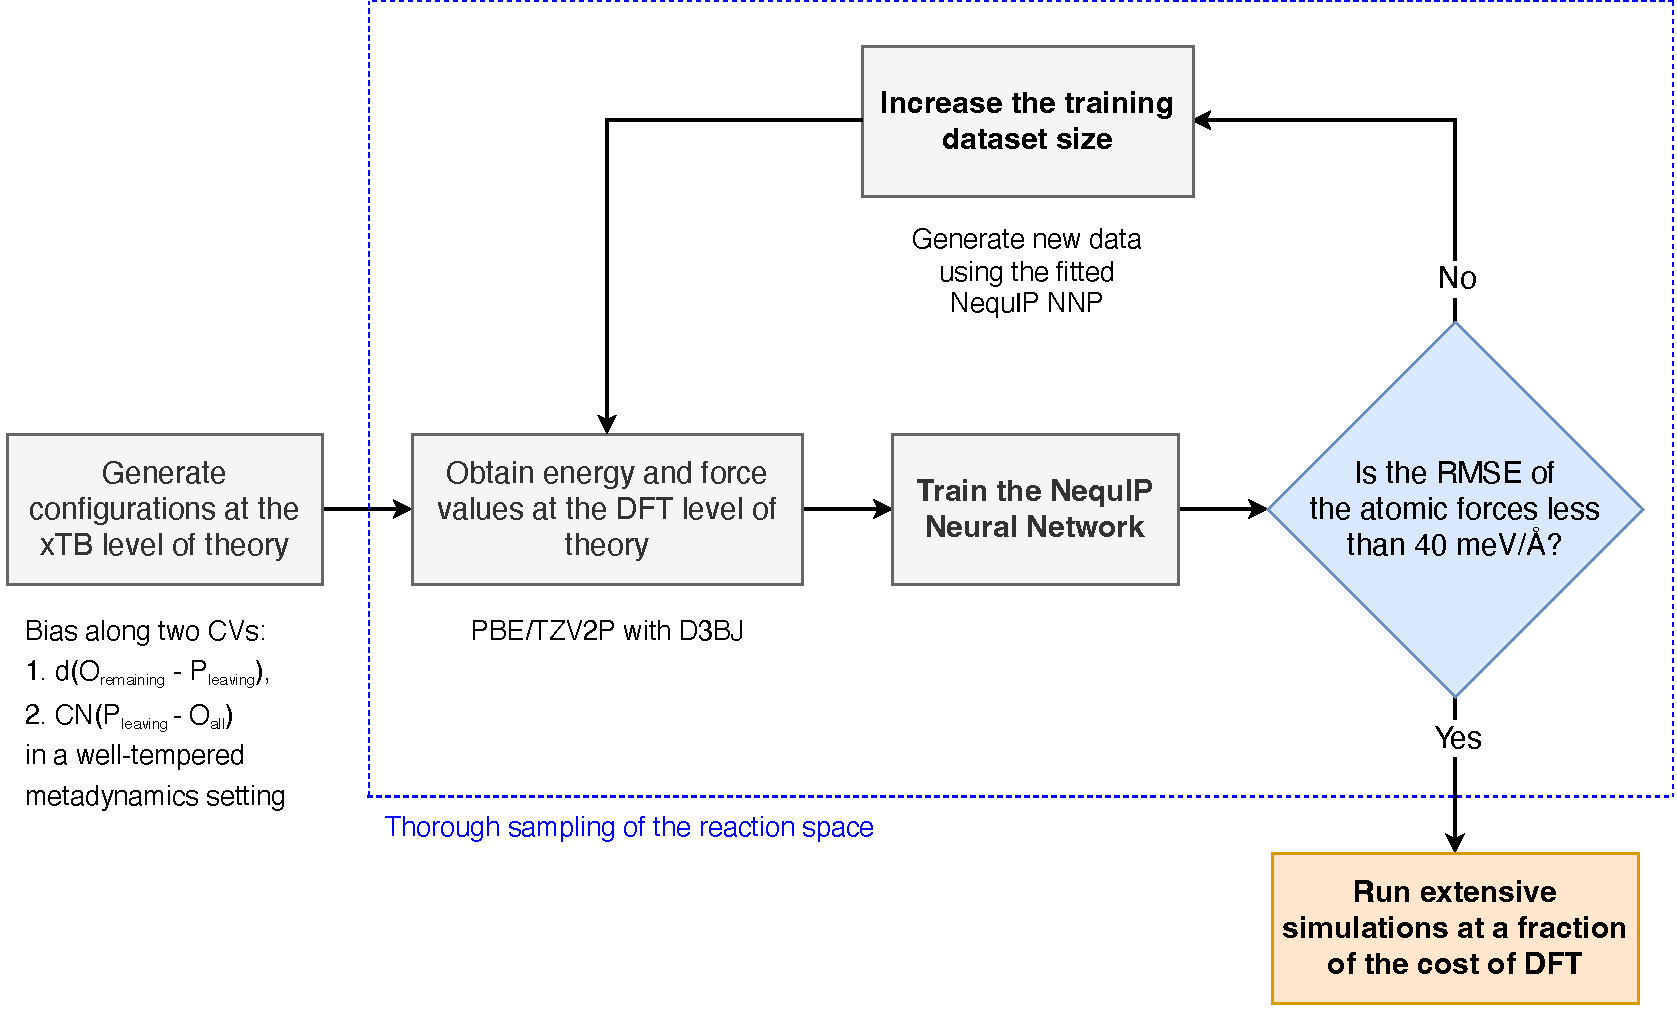
\includegraphics[width=0.95\textwidth]{Figures/3_Computational_details/workflow_diagram_updated.pdf}
    \caption{Iterative training of the NequIP neural network potential.}
    \label{fig:iterative-training}
\end{figure}



\subsubsection{Selection of configurations for training and testing}
The important part of the iterative training is the selection of the configurations that will be used to train the neural network. To construct a representative and diverse dataset for training the neural network potential, configurations were selected from a metadynamics trajectory using a density-aware sampling strategy. The raw data were extracted from a COLVAR file generated during the enhanced sampling simulations. Each configuration in this file corresponds to a simulation snapshot, annotated with a time index and two collective variables (CVs): the distance $d(\mathrm{O}_\text{remaining} - \mathrm{P}_\text{leaving})$ and the coordination number $\mathrm{CN}(\mathrm{P}_\text{leaving} - \mathrm{O}_\text{all})$.

The two CVs were combined into a two-dimensional feature space $\mathbf{X} = (d, \mathrm{CN})$, which serves as the basis for sampling. This feature space often exhibits regions of highly non-uniform data density, due to the biased nature of metadynamics sampling. To account for this, a density-aware sampling method was employed to select configurations for training and testing that maintain good coverage across the feature space.

The selection procedure proceeds as follows:
\begin{enumerate}
    \item A user-defined number of samples is specified.
    \item K-means clustering is applied to the feature space to partition it into a number of clusters, $k$. The number of clusters is determined heuristically as $k = \max\left(10, \; \min\left(\left\lfloor \frac{N}{50} \right\rfloor, \left\lfloor \frac{n_\text{samples}}{10} \right\rfloor \right)\right)$, where $N$ is the total number of configurations and $n_\text{samples}$ is the desired number of samples.
    \item The number of points sampled from each cluster is proportional to its size, ensuring that denser regions do not dominate the dataset. A minimum of one sample is taken from each non-empty cluster.
    \item Within each cluster, a fixed number of configurations are randomly selected using a deterministic random seed to ensure reproducibility.
    \item After the training set is selected, the remaining configurations are used to construct the test set, following the same density-aware procedure while ensuring no overlap with the training configurations.
\end{enumerate}

This approach results in a training and test dataset that closely mirrors the overall distribution of the CVs while ensuring that underrepresented regions of the feature space are adequately sampled. The final output consists of two lists of snapshot indices corresponding to the selected training and test configurations, along with their respective CV values. These snapshots were then extracted from the trajectory files for use in model training and evaluation. The pseudo-code for the density-aware sampling algorithm is provided in Algorithm \ref{alg:density_aware_sampling}.



\subsubsection{First round}
In the first round of training of the neural network potential, the model was trained on a small dataset consisting of 4,000 configurations. The configurations were obtained from the very first exploration of the configuration space at 300 K using the GFN1-xTB level of theory as described in Section \ref{subsec:xtb-exploration-of-configuration-space}. The enhanced sampling simulations were biased along the CV\textsubscript{1} and CV\textsubscript{2}. No restraints were applied to the system. The training was performed using the hyperparameters described in Section \ref{subsec:iterative-training-of-the-neural-network-potential}.



\subsubsection{Second round}
In the second round of training, the model was trained on a larger dataset consisting of 8,000 configurations. The additional configurations were obtained from the second round of exploration of the configuration space driven by the NNP obtained after the first round of training.

To run the simulations with the NNP, LAMMPS package \citep{thompsonLAMMPSFlexibleSimulation2022} compiled with PLUMED 2.9.3 \citep{tribelloPLUMED2New2014} and pair\_nequip \citep{MirgroupPair_nequip} was used. The simulations were performed for 100 ps in the NVT ensemble at 300 K. The temperature was controlled by Nos\'e-Hoover thermostat \citep{noseUnifiedFormulationConstant1984, hooverCanonicalDynamicsEquilibrium1985} with a time constant of 50 fs. The biasing potential was applied to the CV\textsubscript{1} and CV\textsubscript{2} every 50 fs with a gaussian hill height of 2 kcal mol\textsuperscript{-1} and a width of 0.07 for each CV. The bias factor was set to 30. The time step for the integration was set to 0.5 fs.

The restraints were applied to CV\textsubscript{2} in order to favour dissociative or associative mechanism of the reaction. The training was performed using the same hyperparameters as in the first round.

\subsubsection{Third round}
In the last round of training, the model was trained on a dataset consisting of 12,000 configurations. The additional configurations were obtained from the third round of exploration of the configuration space driven by the NNP obtained after the second round of training. The simulations were performed for 500 ps in the same setup as in the second round. The only difference is that the temperature in this round was set to 320 and 340 K to explore the configuration space at higher temperatures. No restraints were applied to the system. The training was performed using the same hyperparameters as in the first round. The final dataset can be seen in Table \ref{tab:full_dataset}.



%%%%%%%%%%%%%%%%%%%%%%%%%%%%%%%%%%%%%%%%%%%%%%%%%%%%%%%%%%%%%%%%%%%%%%%%%%%%%%%%

\section{Production runs at different temperatures}

%%%%%%%%%%%%%%%%%%%%%%%%%%%%%%%%%%%%%%%%%%%%%%%%%%%%%%%%%%%%%%%%%%%%%%%%%%%%%%%%

\section{Validation of the transition states}

%%%%%%%%%%%%%%%%%%%%%%%%%%%%%%%%%%%%%%%%%%%%%%%%%%%%%%%%%%%%%%%%%%%%%%%%%%%%%%%%

\section{Lifetime of the transition states}

%%%%%%%%%%%%%%%%%%%%%%%%%%%%%%%%%%%%%%%%%%%%%%%%%%%%%%%%%%%%%%%%%%%%%%%%%%%%%%%%

\section{Data analysis and visualisation}